\def \ti{\textit}
\def \bf{\textbf}

\chapter{Introduzione}
	\label{cap:intro}
	
\section{Scopo del progetto}
	\label{sec:scopo}

Il progetto sviluppato in questi mesi per il corso di ``Sicurezza Informatica e Internet'' si propone come scopo quello di realizzare un'applicazione che permetta di gestire un documento cartaceo in forma sicura.
In particolare questo significa che chi utilizza tale sistema deve essere in grado di
\begin{itemize}
	\item compilare un foglio con informazioni sensibili;
	\item cifrare tutto o alcune parti del foglio al fine di poterlo inviare a chiunque voglia;
	\item decifrare il contenuto di un documento ricevuto da un'altra persona.
\end{itemize}
Lo scopo ultimo è dunque quello di abilitare l'utilizzatore ad inviare ad un gruppo di persone il documento che ha appena creato. Tuttavia durante il trasferimento (funzione che non compete a questa applicazione) può succedere che il documento possa venire alterato in alcune sue parti se non si utilizzano canali sicuri; moltissime truffe avvenute in passato si sono basate su questa vulnerabilità. Dunque uno degli scopi è quello di garantire con opportune tecniche basate su crittografia asimmetrica che il documento cartaceo resti robusto ed inattaccabile qualunque sia il canale di comunicazione che l'utente finale sceglie per l'invio.
Nel caso di questo progetto, l'elaborazione riguarda documenti cartacei, quindi non è possibile archiviare le informazioni sensibili in una qualche struttura dati. La sfida più importante è quella di trasportare insieme al documento stampato le informazioni segrete.
Questo apre una serie di problematiche legate alla gestione delle informazioni che sono in formato digitale nella fase di composizione e diventano analogiche nella fase di acquisizione di un documento spedito (che può essere stampato e acquisito più volte durante il percorso - per esempio via fax).
La tecnologia migliore per il trasporto dei dati su immagini è rappresentata dal \emph{QR-Code}, un particolare tipo di codice a barre 2D che può contenere al suo interno una discreta quantità di informazioni.
I dati possono essere riletti utilizzando algoritmi di riconoscimento robusti che hanno raggiunto nel tempo un elevata maturità.
Nell'ambito di questo progetto i QR-Code sono stati utilizzati sia per memorizzare le informazioni cifrate, sia per apporre una firma digitale al documento intero. Si risponde così alle esigenze di mantenere segreti alcuni contenuti e di rendere il documento robusto alle manipolazioni esterne.

Un'altra funzionalità importante che rientra negli scopi di questa applicazione, è quella di creare una gerarchia tra gli utenti che accedono al servizio. 
Può capitare, infatti, di voler pubblicare un certo documento e di voler permettere solo a pochi eletti di accedere alle informazioni cifrate. Questo implica che nel sistema si avranno utenti con livelli di privilegio diversi dove ognuno di questi può decifrare e leggere solo le informazioni adeguate al suo livello.
In questo caso la soluzione più ovvia potrebbe essere quella di pubblicare versioni diverse dello stesso documento oscurando opportunamente sulle diverse copie le informazioni che si vogliono tenere segrete a ciascun gruppo. Questo processo può risultare lungo, macchinoso e poco sicuro: è possibile, infatti, che qualche copia possa finire al destinatario sbagliato se non si prendono opportune precauzioni.
Ci si è quindi occupato di realizzare un sistema dove la cifratura viene effettuata con chiavi speciali (che da ora in poi verranno chiamate \textbf{chiavi di livello}), le quali vengono distribuite solo agli utenti che hanno un \textbf{livello di fiducia} (o \textbf{Trust~Level}) adeguato. In questo caso un Trust~Level basso corrisponde ad un basso livello di privilegio, mentre un Trust~Level alto garantisce l'accesso a tutte le informazioni cifrate con le chiavi di livello più basso.

Riassumendo quindi, per quanto riguarda le funzionalità principali, il sistema dovrebbe permettere di:
\begin{itemize}
	\item compilare un documento contenente qualsiasi tipo di informazione;
	\item cifrare in tutto o in parte il documento appena scritto;
	\item allegare le informazioni cifrate al documento stesso così che il o i destinatari possano leggerlo;
	\item firmare il documento in modo tale che il mittente non possa ripudiarne la provenienza e i destinatari possano accorgersi di eventuali manomissioni durante il trasferimento;
	\item specificare diversi livelli di privilegio gerarchici per la lettura delle informazioni.
\end{itemize}

\section{Tecnologie Utilizzate}
	\label{sec:tecnologie}
Gli obiettivi appena illustrati, danno un'idea delle tante problematiche che l'applicazione deve affrontare. Per questo sono molte le tecnologie che sono state messe in gioco. Nel seguito di questo paragrafo verranno spiegate quelle utilizzate maggiormente.

\subsection{Strumenti di sviluppo}
Per quanto riguarda gli strumenti, si è fatto uso di
\begin{itemize}
		\item \textbf{Eclipse Luna} come IDE per la gestione del progetto e dei file sorgente;
		\item \textbf{Apache Maven v2.2} per la gestione delle dipendenze e del ciclo di vita dell'applicazione;
		\item \textbf{Git} per il \emph{versioning} e la condivisione dei sorgenti nel team (in particolare si è usato un repository pubblico\footnote{Per certi versi si è seguito il principio di \emph{Auguste Kerckhoffs} secondo cui ``\emph{in un sistema crittografico è importante tener segreta la chiave, non l'algoritmo di crittazione}''.} su \emph{GitHub} come piattaforma online di condivisione\footnote{Link del repository:\url{https://github.com/WAFcoding/ProgettoSicurezza.git}});
\end{itemize}

\subsection{Linguaggio e librerie utilizzate}
In questo progetto è stato utilizzato \texttt{Java} come linguaggio di programmazione principale. I motivi di questa scelta ricadono principalmente su:
\begin{itemize}
	\item il paradigma Object-Oriented che ha permesso l'utilizzo di architectural e creational pattern  per risolvere le problematiche più comuni, come Façade, Factory Method, Abstract Factory, DAO e Singleton che sono stati ampiamente utilizzati nello sviluppo;
	\item l'alta manutenibilità del codice;
	\item la portabilità su altre piattaforme diverse da quella di sviluppo;
	\item la grande quantità di librerie presenti a supporto degli obiettivi descritti prima.
\end{itemize}

Per quanto riguarda invece i singoli moduli del software sviluppato, si sono utilizzati diversi framework e librerie.
Per la parte di sicurezza c'è:
\begin{itemize}
	\item \texttt{JCA/JCE} (Java~Cryptographic~Architecture/Java~Criptographic~Extension) come framework e provider dei principali algoritmi di cifratura, firma e hashing;
	\item \texttt{BouncyCastle} che si integra con JCA/JCE  e fornisce un maggior numero di algoritmi di cifratura e firma nonché funzioni di generazione di certificati; 
\end{itemize}

Per il modulo di elaborazione dei documenti:
\begin{itemize}
	\item \texttt{ImageMagik} per la manipolazione delle immagini dei documenti acquisiti per la decodifica;
	\item \texttt{ZXing} per la generazione e lettura di QR-Code (in generale supporta molti tipi di codici a barre sia 1D che 2D);
	\item \texttt{iTextPDF} per la generazione di documenti ad alta risoluzione ed il posizionamento preciso di testo e QR-Code nel documento;
	\item \texttt{Tesseract} ed in particolare il wrapper Java \texttt{Tess4J} per il recupero del testo dopo la scansione dei documenti.
\end{itemize}

Per la parte di persistenza invece si è fatto uso di:
\begin{itemize}
	\item \texttt{MySQL} come database relazionale per il sistema di \emph{provisioning} delle chiavi e la gestione degli utenti;
	\item \texttt{SQLite} per la gestione dei dati locali di ogni singolo utente (sotto forma di database cifrato);
	\item \texttt{Hibernate} come framework per la gestione dei database (MySQL e SQLite), ed in particolare il modulo \texttt{ORM} (Object-Relational~Mapping).
\end{itemize}

\section{Le principali tecnologie}
Di seguito una breve panoramica dello stato dell'arte delle tecnologie utilizzate maggiormente nello sviluppo di questo progetto.
Si analizzeranno in particolar modo il \textbf{QR-Code} e l'\textbf{OCR}.
\subsection{QR-Code}
	\label{subsec:qrcode}
Il \emph{QR-Code} (Quick~Response~Code in virtù del fatto che il codice fu sviluppato per permettere una rapida decodifica del suo contenuto) è un codice a barre bidimensionale, ossia a matrice, composto da moduli neri disposti all'interno di uno schema di forma quadrata. Viene impiegato per memorizzare informazioni generalmente destinate a essere lette tramite un dispositivo mobile. In un solo codice QR possono essere contenuti oltre $7089$ caratteri numerici o $4296$ alfanumerici.
Il QR-Code fu sviluppato nel $1994$ dalla compagnia giapponese \emph{Denso~Wave} allo scopo di tracciare le componenti di automobili nelle fabbriche della Toyota. Vista la capacità del codice di contenere più dati di un codice a barre venne in seguito utilizzato per la gestione delle scorte da diverse industrie.
Tuttavia essendo un codice che deve essere riportato su un documento cartaceo, può subire dei danni che possono provocare degli errori nella seguente lettura.
Per questo viene utilizzato il codice Reed-Solomon per la rilevazione e correzione d'errore che permette di ricostruire i dati persi, ripristinando, durante la decodifica, fino al $30\%$ delle informazioni codificate.

	\begin{center}	
		\begin{figure}[H]
		\centering
		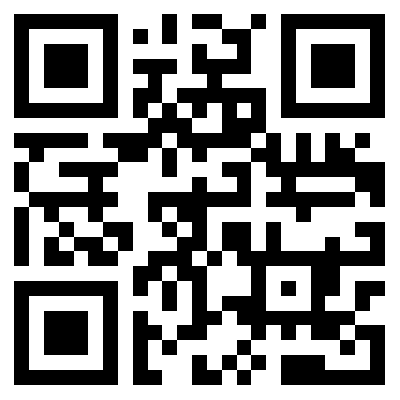
\includegraphics[scale=0.9]{Immagini/qrcode}
		\caption[Esempio di QR-Code]{Un esempio di QR-Code.}
		\label{fig:usecase}
		\end{figure}
	\end{center}

\subsection{OCR}
	\label{subsec:ocr}
La parola \emph{OCR} (Optical~Character~Recognition) descrive una classe di sistemi di riconoscimento ottico dei caratteri.
Gli OCR sono programmi dedicati alla conversione di un'immagine contenente testo, solitamente acquisite tramite scanner (come nel caso di questo progetto), in testo digitale modificabile con un normale editor. Il testo può essere convertito in formato \texttt{ASCII} semplice, \texttt{Unicode} o, nel caso dei sistemi più avanzati, in un formato contenente anche l'impaginazione del documento.
L'OCR è un importante campo di ricerca dell'intelligenza artificiale, della visione artificiale e del pattern recognition, legati al riconoscimento delle immagini.
I sistemi OCR per funzionare correttamente richiedono una fase di ``addestramento''. Durante questa fase al sistema vengono forniti degli esempi di immagini col corrispondente testo in formato ASCII o simile in modo che gli algoritmi si possano calibrare sul testo che usualmente andranno ad analizzare. Gli ultimi software di OCR utilizzano algoritmi in grado di riconoscere i contorni e in grado di ricostruire oltre al testo anche la formattazione della pagina.
Gli OCR possono essere usati per riconoscere:
\begin{itemize}
	\item caratteri stampati, per i quali gli algoritmi noti hanno un tasso di errore del $1\%$;
	\item scrittura a mano libera, problema tutt'altro che risolto, per la quale gli algoritmi hanno tassi di accuratezza dell'$80\%$ - $90\%$;
	\item caratteri in corsivo, che è un campo in fase di studio, per il quale si hanno tutt'oggi risultati poco soddisfacenti a livello di accuratezza. 
\end{itemize}

	\begin{center}	
		\begin{figure}[H]
		\centering
		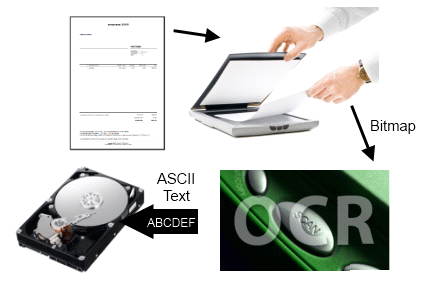
\includegraphics[scale=0.9]{Immagini/ocr}
		\caption[OCR]{Processo da seguire per utilizzare un sistema OCR.}
		\label{fig:usecase}
		\end{figure}
	\end{center}